\section{Wormhole}

In order to allow more interesting manifolds than a few that I hard code in, I plan to implement connected sums of manifolds. Unfortunately, almost none of the well-known manifolds can be smoothly connected without changing their metrics. In order to facilitate this, I have found a class of manifolds that can be used as intermediates to smoothly connect two manifolds of constant curvature, and which allows geodesics to be easily calculated. I call them wormholes.

The wormhole is topologically $S^2 \times \mathbb{R}$, but with a different metric.

Given $p_1, p_2 \in S^2 \times \mathbb{R}$,

$p_1 = (s_1,r_1)$

$p_2 = (s_2,r_2)$

Let $S$ be the great circle containing $s_1$, $s_2$.

$p_1, p_2$ are in the slice $S \times \mathbb{R}$ of $S^2 \times \mathbb{R}$.

Let $\theta_1, \theta_2 \in S^1$ be $s_1, s_2$ under the inverse inclusion map.

$p_1 = (\theta_1,r_1)$

$p_2 = (\theta_2,r_2)$

$S \times \mathbb{R}$ corresponds to a quotient space of the half-plane model of $\mathbb{H}^2$ by $(\theta,r) \mapsto (e^{k\theta} \cos r, e^{k\theta} \sin r)$ where $k$ is a constant depending on the quotient space.

The two semicircles in the picture are identified to form the quotient.

\begin{figure}[h]
\subfigure[$S^2 \times \mathbb{R}$]{
	\label{fig:S2xR}
	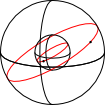
\includegraphics[scale=0.5]{../images/S2xR.png}
}
\subfigure[Half Plane]{
	\label{fig:halfplane}
	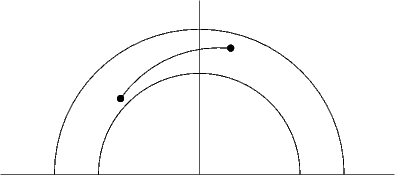
\includegraphics[scale=0.3]{../images/HalfPlane.png}
}
\subfigure[Radial Lines]{
	\label{fig:radiallines}
	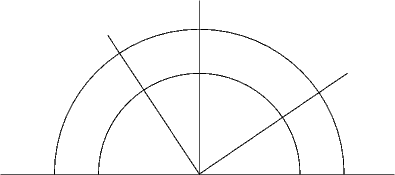
\includegraphics[scale=0.3]{../images/RadialLines.png}
}
\end{figure}

Find a geodesic in $\mathbb{H}^2$ that connects $p_1$ and $p_2$, and map it back to $S \times \mathbb{R} \subseteq S^2 \times \mathbb{R}$.

Radial lines are curves of constant curvature. These map to closed loops. The angle of the lines controls how the curvature and diameter relate allowing connection to a space of a specific curvature.
